\externaldocument[I-]{MaxHughesThesis}

The output of the GEANT4 was used to fit the data spectra. 
First, however, it had to be processed. 

\section{Simulation Results Processing}
After the events were done, the simulation data was processed further. 
Much like the experimental data, the simulated data had to be filtered.
The energy absorbed in the implant detector was filtered by the energy absorbed in the outer four gamma detecters in the simulation.

The filtered data was seperated into two parts:
Absorbed energy in the implant detector only orginating from the electron.
Absorbed energy in the implant detector with some contribution from the gamma ray.
These energies were built into two different histograms.
These two histograms had the detector resolution applied to it. 

The convolution function was

\begin{equation}
	\sigma = A\sqrt{E}
	\label{eq:convo}
\end{equation}

where $\sigma$ was the energy resolution, $E$ the energy, and $A$ a constant found through a calibration.

\subsubsection{Pile-up Modelling}
After the convolution, the simulation data was sent through a simulation to model pile-up.
The model used for the CsI(Na) signals was a linear rise and then an exponential decay.
The linear part went from 0 to 1 over 100 ns. 
The exponential piece started at 100 ns at 1 and decayed with a $\tau$ of 760 ns.
This analytic equation was scaled up or down to whatever energy was sampled.
It was then fed into a model of trapezoidal filter of PIXIE. 
The math was the same as described in the chapter on data aquisition.


This model was tuned on calibration data. 
A run was taken of $^{137}$Cs at 25000 counts per second.
A 2000 counts per second $^{137}$Cs run was used as a background and subracted off.
Then, samples of the background-subtracted spectrum were taken up to the end of the 661 keV peak.
Monte Carlo methods were used to model the time difference between two samples.
If the two samples fell within the pile-up window, then the piled-up signal models were fed into the trapezoidal filter.
The calculated pile-up energy was saved to a histogram.
If the two samples did not fall with in the pile-up window, then they were not fed into the filter model and just filled into the histogram.
The paremeters were adjusted until the generated pile-up matched the measured pile-up in the spectrum.
The results of the tuning is seen in figure \ref{fig:pileuptune}

\begin{figure}[!htb]
	\centerline{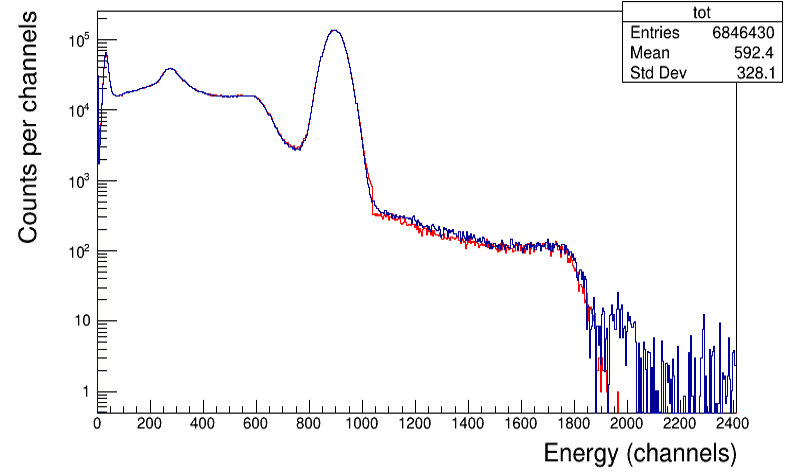
\includegraphics[width=0.78\textwidth]{PileUpTuningThesis.png}}
	\caption{The tuning of the pile-up.
		 The input spectrum is in blue.
		 It was sampled up to 1000 channels.
		 The generated spectrum is in red.}
	\label{fig:pileuptune}
\end{figure}

\section{Calibration}
In order to properly fit the energy spectrum, a calibration of the CsI(Na) detector had to be done.
Several different energy lines were used to find the calibration and the energy resolution function.
The lines were the 1.173228 MeV and 1.332492 MeV gammas from a $^{60}$Co source, the 0.661657 MeV gamma ray from a$^{137}$Cs source, and the 0.511 MeV and 1.274527 MeV gamma rays from a $^{22}$Na source.
These gamma rays were fitting with a gaussian and a background.
The background varried from a linear background, a quadratic background, and an error function background.
For the $^{60}$Co, both peaks were fit at once.
These different background gave slightly different results for the centroids and the widths of the gaussians.
The different widths and centroids were taken as a systematic error.
From the centroids, the calibration for each detector was calculated and shown in equation \ref{eq:cal}

\begin{equation}
	C = G * E + b
	\label{eq:cal}
\end{equation}

where $C$ is the location of the peak in ADC channels, $G$ the gain in channels/keV, and b the offset in channels.
The widths of the peaks were calibrated with the gain and plotted vs energy.
Then, equation \ref{eq:convo} was fit to the results in order to determine $A$.

\section{Fitting Procedure}
The simulation described above were only part of what was needed.
Other simulations included in the fit had the phase space times corrections times or divided an additional factor of the total energy of the electron.
The simulations were all convoluted and filtered as described above.

\subsection{Data Processing}
The data was processes from the TTrees described in the previous section.
The energy spectrum of the implant detector was put in coincidence with the 4 gamma detectors.
The energy cuts of the gamma detectors were the same as in the life-time measurement.
There was a time difference condition as well.
For this measurement, the time difference between a beta event and a gamma event had to be between -300 and 24 ns.
Then, a 2-D histogram was built, with energy on one axis and time since last beam on on there other.
Since afterglow causes an effect that looks like a gain shift, different time cuts of equal statistics were taken from this 2-D histogram. 
These time cuts were then fit. 
The gain was left as a free parameter to counteract this afterglow effect.

\subsection{Fit Function}
The fit function used was as follows.
First, the x axis of the data was read.
This number was in ADC units, so equation \ref{eq:cal} was used to turn this number into energy in keV.
For the fitting, the gain $G$ was left as a free parameter, but the offset $b$ was set from the calibration.

\begin{equation}
	H(E) = A * (f(E)_{nosum} * S(E,b_{wm}) + f(E)_{summing}) + B*p(E)
	\label{eq:betafit}
\end{equation}

where $A$ is the normalization, $B$ the level of pile-up, $E$ the energy, $b_{wm}$ the weak magnetism, $S(E,b_{wm})$ the shape factor, $f(E)_{nosum}$ the output of the GEANT4 simulation without any energy summing between the gamma and beta, and $f(E)_{summing}$ the output of the GEANT4 simulation with energy summing.
The free parameters here are $A$, $B$, and $b_{wm}$.

\subsection{Fit details}
The fit was done run by run.
First a prefit for each section was done to calibrate the energy.
Then, two endpoints in keV were used for the fit.
The fitting function with a fixed offset was fit using a maximum likelyhood method.
The resulting $b_{wm}$ was recorded.

The gain used for these fits was 10.05 ADC channels.
The end points for the calibration pre-fit were 540 channels to 7000 channels.
The calibrated end points were 800 keV to 7500 keV. 
 
